\documentclass{ltjarticle}

\usepackage{graphicx}
\usepackage{hyperref}
\usepackage{subcaption}
\usepackage{xcolor}
\usepackage{amssymb}
\usepackage{amsmath}
\usepackage{authblk}

\renewcommand{\figurename}{Figure}

\title{Computer Vision-based Comparison of Woodblock-printed Books and its Application to Japanese Pre-modern Text}

\author[1,3]{Thomas Leyh}
\author[2,3]{Asanobu Kitamoto}
\affil[1]{University of Freiburg}
\affil[2]{ROIS-DS Center for Open Data in the Humanities}
\affil[3]{National Institute of Informatics}

\date{}

\usepackage[backend=biber,style=alphabetic,sorting=nyt]{biblatex}
\addbibresource{references.bib}

\begin{document}

\maketitle

\section{Introduction}

Digital Humanities have potential to reduce the complexity of bibliographical study by developing technical tools to support comparison of books. So far, the effort has been mainly put into text-based methods on large corpora of literary text. However, the emergence of large image datasets, along with the recent progress in Computer Vision, opens up new possibilities for bibliographical study without text transcriptions. This paper describes the technical development of such an approach to Japanese pre-modern text, and in particular to Bukan, which is a special type of Japanese woodblock-printed book.

The authors have been approaching this problem in the past. \cite{kitamoto2018} proposed the concept of “differential reading” for visual comparison. Furthermore, \cite{hakim2019} proposed “visual named-entity recognition” for identifying family crests, using them for a page-by-page matching across different versions. This paper is a follow-up of these works and proposes a keypoint-based method for the page-by-page matching, additionally yielding an option for highlighting differences. 

\section{Dataset}

This work is mainly concerned with extracting information from a specific type of book: 武鑑---Bukan. These are historic Japanese books from the Edo period (1603-1868). Serving as unofficial directories of people in Tokugawa Bakufu (the ruling government in Japan), they include a wealth of information about regional characteristics such as persons, families and other key factors. See figure~\ref{fig:shuugyokubukan006} for an example. These books were created with woodblock-printing. Because the same woodblock has been reused for many versions of the book---sometimes with minor modifications---visual comparison can reveal which part of the woodblock was modified or has degraded.

\begin{figure}
    \centering
    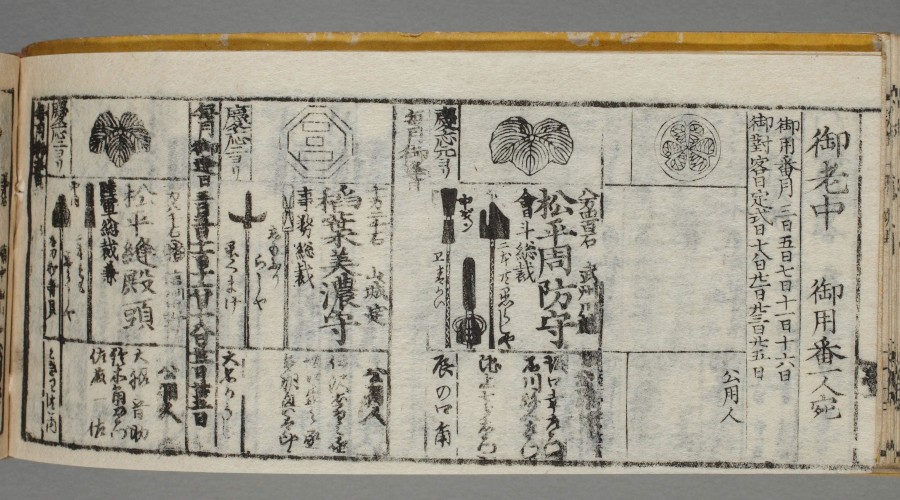
\includegraphics[width=\textwidth]{200019649_00006}
    \caption[Shūgyoku Bukan (袖玉武鑑), page 6]{Shūgyoku Bukan (袖玉武鑑) from 1867, page 6; showing names, descriptions, family crests and procession items. Especially interesting are the blank areas on the right, because in other edition they contain text.}
    \label{fig:shuugyokubukan006}
\end{figure}

ROIS-DS Center for Open Data in the Humanities and the National Institute of Japanese Literature are offering 381 of these Bukan as open data \cite{codh2018bukan}. The original images have a width of $5616$ and height of $3744$ pixels. From the open data we created a derived dataset using the following preprocessing methods. Under the assumption that this task (1) does not require this level of detail, (2) does not require information about color and (3) only compares the actual pages, not the surrounding area, all scans are resized by $25\%$, converted to grayscale and finally cropped, resulting in an image shape of $990 \times 660$ pixels. If there are two book pages per scan, they were additionally split at their horizontal center.

\section{Method}

Using an approach based on Computer Vision, two techniques were applied:

\begin{enumerate}
    \item “Keypoint Detection and Matching” for finding the same features in different images.
    \item “Projective Transformations” for comparing two different images regardless of their original orientation.
\end{enumerate}

We used the \emph{OpenCV} software library.\cite{opencv_library}

\subsection{Keypoint Matching}

Keypoint Detection\cite[Ch.4]{szeliski2010computer} is about finding points of interest in an image that are most noticeable and give a unique description of the local area surrounding them. Computer Vision research produced various kinds of keypoints, most prominently SIFT\cite{lowe2004sift}. For evaluating the performance of these algorithms, 12 prints of the Shūchin Bukan (袖珍武鑑) were manually annotated, in total around 1800 pages, holding information about the position of matching pages.

\begin{figure}
    \centering
    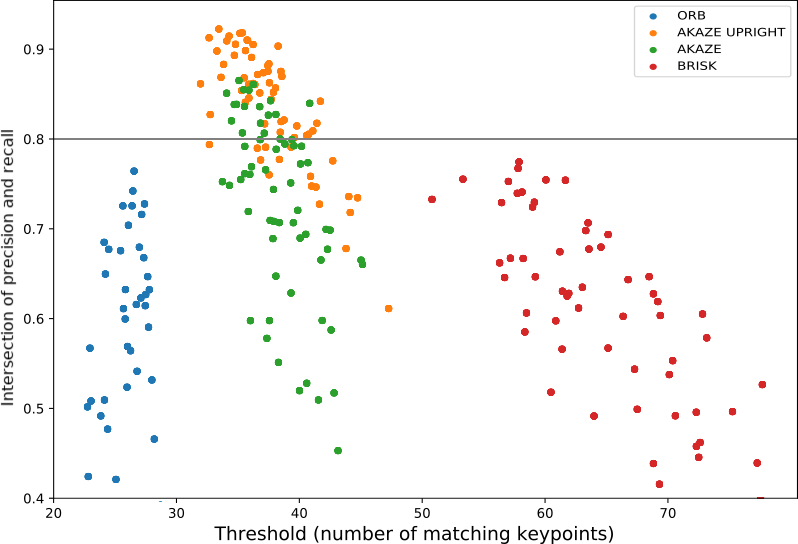
\includegraphics[width=\textwidth]{keypointevaluation}
    \caption[Scatterplot of keypoint matching performance]{Scatterplot for evaluating keypoint matching performance for each book pair of the annotated data for different keypoint algorithms. Each dot represents the precision-recall-intersection of a book pair (y-axis) against a threshold on the number of matching keypoints (x-axis). All points above the gray horizontal line at $0.8$ are considered “good enough” by the authors. There is a general tendency in favor of AKAZE UPRIGHT discernible.}
    \label{fig:keypoint-evaluation}
\end{figure}

Using these annotations, six keypoint algorithms were empirically evaluated\footnote{ORB\cite{rublee2011orb}, AKAZE\cite{alcantarilla2011fast}, AKAZE without rotational invariance (UPRIGHT), BRISK\cite{leutenegger2011brisk}, SIFT, SURF\cite{bay2006surf}} by trying to match over all possible page combinations. This produces a list of similar keypoint pairs for each combination. The number of these pairs is then interpreted as score for the similarity of two pages. The decision about an actual page match is made by thresholding on this score. At this point, AKAZE UPRIGHT has the best performance with an average precision and recall of around $0.8$ with respect to the threshold. See figure~\ref{fig:keypoint-evaluation} for further details.

\subsection{Projective Transformations}

\begin{figure}
    \centering
    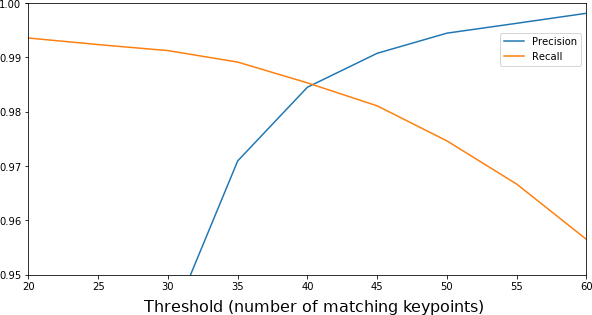
\includegraphics[width=0.9\textwidth]{ransacperformance}
    \caption[RANSAC performance]{Applying RANSAC on the keypoint matches from AKAZE UPRIGHT results in better classification results: For all page pairs, precision and recall (y-axis) by threshold on the number of matching keypoints (x-axis) is above $0.95$ and much more stable regarding the threshold.}
    \label{fig:ransac}
\end{figure}

For images, a Projective Transformation (or Homography) is a matrix $\mathbf{H} \in \mathbb{R}^{3 \times 3}$ for transforming homogeneous coordinates $\mathbf{H}\vec{x} = \vec{y}$ ($\vec{x}$ and $\vec{y}$ are interpolated pixel coordinates). This operation results in linear transformations like translation and rotation, but also changes in perspective.\cite{marschner2015fundamentals} For finding such a transformation from matching keypoints, the heuristic \emph{Random Sample Consensus} (RANSAC) algorithm is commonly used.\cite{fischler1981random} Basically, a random subset of matching keypoints is chosen, using this to compute a transformation and calculating an error metric. By iteratively using different random subsets, eventually the transformation with the smallest error is picked.

The benefit is twofold: First, the algorithm implicitly uses spatial information of the matching image candidates to filter out false positives, thus greatly boosting the matching performance. Precision and recall are close to their maximum of $1.0$, see figure~\ref{fig:ransac}. Secondly, it directly yields the transformation matrix $\mathbf{H}$, enabling the creation of image overlays for visualizing the differences. Looking at the perspective components of $\mathbf{H}$, additional filtering is done\footnote{By asserting that $|\mathbf{H}_{1,3}| \leq 0.001$ and $|\mathbf{H}_{2,3}| \leq 0.001$.}, removing even more of the remaining false positives.

\section{Discussion}

This two-step-pipeline archives high precision and recall when looking for similar pages of different book editions. Performance seems to be robust with respect to most parameters. For classifying two pages as match, the number of matching keypoints is important since it is acting as a score. By preserving this value it is possible to rank page pairs by visual similarity. Furthermore, a threshold can be set dynamically, even after the computation of keypoint pairs. Assuming semi-automatic application with a human assessing the results, recall is of higher importance, thus a low threshold of around $40$ is recommended, but can be adjusted any time. See again figure~\ref{fig:ransac} for the slope of the recall curve.

\begin{figure}
    \centering
    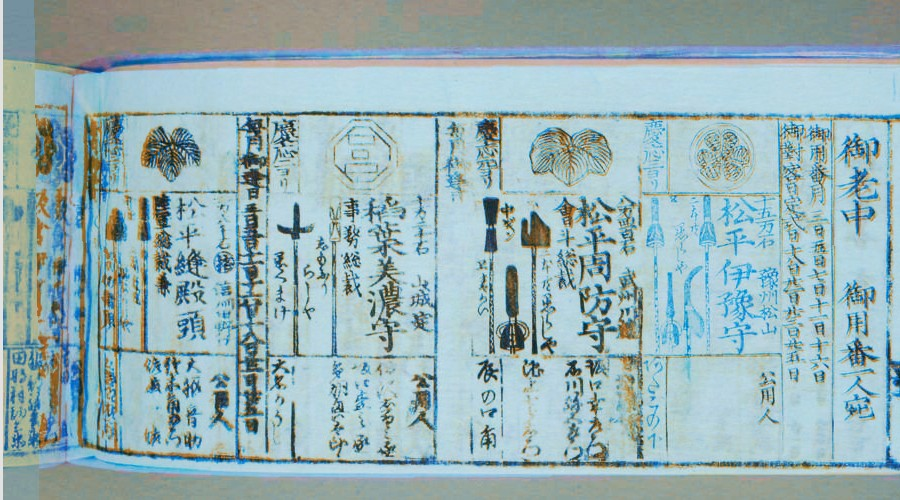
\includegraphics[width=\textwidth]{200019646_00006}
    \caption[Visualizing page differences]{Visualizing page differences between two prints of the Shūchin Bukan (袖珍武鑑) from 1867. Differences are indicated by \textcolor{blue}{blueish} and \textcolor{red}{reddish} coloring.}
    \label{fig:page-compare}
\end{figure}

This can serve as base for building a comparison browser: A scholar in the humanities can browse a book while getting information about similar pages. Differences between pages can be visualized at any time, similar to figure~\ref{fig:page-compare}. This is expected to lessen her burden when examining numerous pages, since small, abstract differences are often hard to discern for the human eye.

\section{Conclusion}

Open Data and digitization are accompanied by new possibilities, especially in the humanities. Here, algorithms from Computer Vision were able to produce excellent results on visually comparing pages and whole books. Especially RANSAC---despite its age---might still hide some of its potential. Current works on e.g. image alignment \cite{shen2019ransac} continue to build upon this method, proving its usefulness.

\printbibliography

\end{document}